\documentclass[oneside,openany,headings=optiontotoc,11pt,numbers=noenddot]{scrreprt}

\usepackage[a4paper]{geometry}
\usepackage[utf8]{inputenc}
\usepackage[T1]{fontenc}
\usepackage{lmodern}
\usepackage[ngerman]{babel}
\usepackage{ngerman}

\usepackage[onehalfspacing]{setspace}

\usepackage{fancyhdr}
\usepackage{fancybox}

\usepackage{rotating}
\usepackage{varwidth}

%Struktogramme
\usepackage[german,curves]{struktex}

\usepackage{pdflscape}
\usepackage{changepage}
\usepackage{graphicx}
\usepackage[bottom]{footmisc}
\usepackage{transparent}
\usepackage{graphbox}
\graphicspath{
	{Pics/PDFs/}
	{Pics/JPGs/}
	{Pics/PNGs/}
}
\usepackage{caption}
\usepackage{wrapfig}
\usepackage{marginnote}
\usepackage{tabularx}
\usepackage{dashrule}
\usepackage{soulutf8}
\usepackage{hhline}
%arydshln suppresses vertical lines in table
%\usepackage{arydshln}
\usepackage{multirow}
\usepackage{enumerate}
\usepackage[hidelinks]{hyperref}
\usepackage{listings}

\usepackage[table]{xcolor}
\usepackage{array}
\usepackage{enumitem,amssymb,amsmath}
\usepackage{interval}
\usepackage{cancel}
\usepackage{stmaryrd}
\usepackage{wasysym}
\usepackage{polynom}
\usepackage{diagbox}
\usepackage{dashrule}
\usepackage{framed}
\usepackage{mdframed}
\usepackage{karnaugh-map}
\usepackage{pdfpages}

\usepackage{blindtext}

\usepackage{eso-pic}

\usepackage{amssymb}
\usepackage{eurosym}

\usepackage[pages=some]{background}
\pagestyle{headings}
\renewcommand{\headrulewidth}{0.2pt}
\renewcommand{\footrulewidth}{0.2pt}
\newcommand*{\underdownarrow}[2]{\ensuremath{\underset{\overset{\Big\downarrow}{#2}}{#1}}}
\setlength{\fboxsep}{5pt}
\newcommand{\explainBelow}[3]{\underbrace{#1}_{\parbox{\widthof{#3}}{\footnotesize\raggedright #2}}}
\newcommand{\explainAbove}[3]{\overbrace{#1}^{\parbox{\widthof{#3}}{\footnotesize\raggedright #2}}}
\newcommand\footnoteref[1]{\protected@xdef\@thefnmark{\ref{#1}}\@footnotemark}


% Codestyle defined
\definecolor{codegreen}{rgb}{0,0.6,0}
\definecolor{codegray}{rgb}{0.5,0.5,0.5}
\definecolor{codepurple}{rgb}{0.58,0,0.82}
\definecolor{backcolour}{rgb}{0.95,0.95,0.92}
\definecolor{deepgreen}{rgb}{0,0.5,0}
\definecolor{darkblue}{rgb}{0,0,0.65}
\definecolor{mauve}{rgb}{0.40, 0.19,0.28}
\colorlet{exceptioncolour}{yellow!50!red}
\colorlet{commandcolour}{blue!60!black}
\colorlet{numpycolour}{blue!60!green}
\colorlet{specmethodcolour}{violet}

%Neue Spaltendefinition
\newcolumntype{L}[1]{>{\raggedright\let\newline\\\arraybackslash\hspace{0pt}}m{#1}}
\newcolumntype{M}{>{\centering\arraybackslash}X}
\newcommand{\cmnt}[1]{\ignorespaces}
%Textausrichtung ändern
\newcommand\tabrotate[1]{\rotatebox{90}{\raggedright#1\hspace{\tabcolsep}}}

%Intervall-Konfig
\intervalconfig {
	soft open fences
}

%Bash
\lstdefinestyle{BashInputStyle}{
	language=bash,
	basicstyle=\small\sffamily,
	backgroundcolor=\color{backcolour},
	columns=fullflexible,
	backgroundcolor=\color{backcolour},
	breaklines=true,
}
%Java
\lstdefinestyle{JavaInputStyle}{
	language=Java,
	backgroundcolor=\color{backcolour},
	aboveskip=1mm,
	belowskip=1mm,
	showstringspaces=false,
	columns=flexible,
	basicstyle={\footnotesize\ttfamily},
	numberstyle={\tiny},
	numbers=none,
	keywordstyle=\color{purple},,
	commentstyle=\color{deepgreen},
	stringstyle=\color{blue},
	emph={out},
	emphstyle=\color{darkblue},
	emph={[2]rand},
	emphstyle=[2]\color{specmethodcolour},
	breaklines=true,
	breakatwhitespace=true,
	tabsize=2,
}
%Python
\lstdefinestyle{PythonInputStyle}{
	language=Python,
	alsoletter={1234567890},
	aboveskip=1ex,
	basicstyle=\footnotesize,
	breaklines=true,
	breakatwhitespace= true,
	backgroundcolor=\color{backcolour},
	commentstyle=\color{red},
	otherkeywords={\ , \}, \{, \&,\|},
	emph={and,break,class,continue,def,yield,del,elif,else,%
		except,exec,finally,for,from,global,if,import,in,%
		lambda,not,or,pass,print,raise,return,try,while,assert},
	emphstyle=\color{exceptioncolour},
	emph={[2]True,False,None,min},
	emphstyle=[2]\color{specmethodcolour},
	emph={[3]object,type,isinstance,copy,deepcopy,zip,enumerate,reversed,list,len,dict,tuple,xrange,append,execfile,real,imag,reduce,str,repr},
	emphstyle=[3]\color{commandcolour},
	emph={[4]ode, fsolve, sqrt, exp, sin, cos, arccos, pi,  array, norm, solve, dot, arange, , isscalar, max, sum, flatten, shape, reshape, find, any, all, abs, plot, linspace, legend, quad, polyval,polyfit, hstack, concatenate,vstack,column_stack,empty,zeros,ones,rand,vander,grid,pcolor,eig,eigs,eigvals,svd,qr,tan,det,logspace,roll,mean,cumsum,cumprod,diff,vectorize,lstsq,cla,eye,xlabel,ylabel,squeeze},
	emphstyle=[4]\color{numpycolour},
	emph={[5]__init__,__add__,__mul__,__div__,__sub__,__call__,__getitem__,__setitem__,__eq__,__ne__,__nonzero__,__rmul__,__radd__,__repr__,__str__,__get__,__truediv__,__pow__,__name__,__future__,__all__},
	emphstyle=[5]\color{specmethodcolour},
	emph={[6]assert,range,yield},
	emphstyle=[6]\color{specmethodcolour}\bfseries,
	emph={[7]Exception,NameError,IndexError,SyntaxError,TypeError,ValueError,OverflowError,ZeroDivisionError,KeyboardInterrupt},
	emphstyle=[7]\color{specmethodcolour}\bfseries,
	emph={[8]taster,send,sendMail,capture,check,noMsg,go,move,switch,humTem,ventilate,buzz},
	emphstyle=[8]\color{blue},
	keywordstyle=\color{blue}\bfseries,
	rulecolor=\color{black!40},
	showstringspaces=false,
	stringstyle=\color{deepgreen}
}

\lstset{literate=%
	{Ö}{{\"O}}1
	{Ä}{{\"A}}1
	{Ü}{{\"U}}1
	{ß}{{\ss}}1
	{ü}{{\"u}}1
	{ä}{{\"a}}1
	{ö}{{\"o}}1
}

% Neue Klassenarbeits-Umgebung
\newenvironment{worksheet}[3]
% Begin-Bereich
{
	\newpage
	\sffamily
	\setcounter{page}{1}
	\ClearShipoutPicture
	\AddToShipoutPicture{
		\put(55,761){{
				\mbox{\parbox{385\unitlength}{\tiny \color{codegray}BBS I Mainz, #1 \newline #2
						\newline #3
					}
				}
			}
		}
		\put(455,761){{
				\mbox{\hspace{0.3cm}
\includegraphics[width=0.2\textwidth]{../../logo.pdf}}
			}
		}
	}
}
% End-Bereich
{
	\clearpage
	\ClearShipoutPicture
}

\geometry{left=2.50cm,right=2.50cm,top=3.00cm,bottom=1.00cm,includeheadfoot}

\begin{document}
	\begin{worksheet}{BGY 16}{Mathematik - Lernbereich 3, Algebraisierung}{Lösung zur Hausaufgabe S.72 Nr. 2 a-c / Nr. 5}
		
		\begin{framed}
			Um von einer Parametergleichung der Form \(E: \vec{x} = \vec{p} + r*\vec{u} + s*\vec{v}\) auf die Koordinatengleichung derselben Ebene \(E: ax_1 + bx_2 + cx_3 = d\) gehen wir wie folgt vor:\\
			\par\noindent
			Zunächst überführen wir die Parametergleichung in ein Gleichungssystem der Form
			\begin{align*}
				x_1 = p_1 + r\cdot{}u_1 + s\cdot{}v_1\\
				x_2 = p_2 + r\cdot{}u_1 + s\cdot{}v_2\\
				x_3 = p_3 + r\cdot{}u_3 + s\cdot{}v_3
			\end{align*}
			Dieses Gleichungssystem versuchen wir mittels dem Gauß-Eliminations-Verfahren in Dreiecks-Form zu überführen, wobei wir Gleichungen für \(r\)  bzw. für \(s\) wollen.
			\begin{tabular}{ll}
				
				\begin{tabularx}{0.4\textwidth}{cl}
					\(x_1\) & \(= p_1 + r\cdot{}u_1 + s\cdot{}v_1\)\\
					\(ex_1 + x_2\) & \(= p_2' + r\cdot u_2'\) \\
					\(E: \mathbf{a}\cdot x_1 + \mathbf{b}\cdot x_2 + \mathbf{c}\cdot x_3\) & \(= \mathbf{d}\)\\
				\end{tabularx}\\
				\multicolumn{2}{c}{oder}\\
				& \begin{tabularx}{0.5\textwidth}{cl}
					\(x_1\) & \(= p_1 + r\cdot{}u_1 + s\cdot{}v_1\)\\
					\(ex_1 + x_2\) & \(= p_2'\ \ \ \ \ \ \ \ \ \  + s\cdot v_2'\)\\
					\(E: \mathbf{a}\cdot x_1 + \mathbf{b}\cdot x_2 + \mathbf{c}\cdot x_3\) & \(= \mathbf{d}\)
				\end{tabularx}
			\end{tabular}\\
			\par\noindent
			Ein alternatives Vorgehen wäre, die Gleichungen nach den Parametern \(r\) und \(s\) umzuformen und diese schrittweise in die restlichen Gleichungen einzusetzen.\\
			\tiny{Hinweis: Dieses Vorgehen macht genau dann Sinn, wenn eine der Gleichungen nur einen Parameter (\(r\) oder \(s\)) enthält.}\normalsize
		\end{framed}		
		\begin{framed}
			\noindent
			\tiny{\color{codegray}\underline{S. 72 Nr. 2 a-c}}\\
			\normalsize\noindent
			Gesucht ist die Koordinatengleichung der Ebene E mit nur ganzzahligen Koeffizienten.\\
			\par
			\textbf{(a)} Gegeben ist die Ebene \(E:\vec{x} = \left(\begin{array}{c}1\\2\\0\end{array}\right) + r\left(\begin{array}{c}1\\0\\1\end{array}\right) + s\left(\begin{array}{c}1\\2\\3\end{array}\right)\)\\
			Wir gehen wie oben erwähnt vor:\\
			\begin{tabularx}{\textwidth}{lll}
				I & \(x_1 = 1 + r + \ s\)\\
				II & \(x_2 = 2\ \ \ \ \ + 2s\) & |\((-2); (:2)\)\\
				III& \(x_3 =\ \ +\ r+ 3s\)\\
				\hline
				II'& \(\frac{1}{2}x_2 - 1 = s\)\\
				& \multicolumn{2}{l}{II' in III einsetzen}\\
				III' & \(x_3 =\ \ +\ r+ 3*(\frac{1}{2}x_2 - 1)\)\\
				& \(x_3 =\ \ + r + \frac{3}{2}x_2 - 3\) & |\((-\frac{3}{2}x_2); (+3)\)\\
				& \(-\frac{3}{2}x_2 + x_3 + 3 = r\)\\
				& \multicolumn{2}{l}{II' \& III' in I einsetzen}\\
			\end{tabularx}
			\begin{tabularx}{\textwidth}{lll}
				I' & \(x_1 = 1 \underbrace{-\frac{3}{2}x_2 + x_3 + 3}_{r} + \underbrace{\frac{1}{2}x_2 - 1}_{s}\)\\
				& \(x_1 = -x_2 + x_3 +3\) & |\((+x_2);(-x_3)\)\\
				& \colorbox{green!10}{\(E_a: x_1 + x_2 - x_3 = 3\)}
			\end{tabularx}\\
			\par
			\textbf{(b)} Gegeben ist die Ebene \(E:\vec{x} = \left(\begin{array}{c}4\\9\\1\end{array}\right) + r\left(\begin{array}{c}1\\2\\0\end{array}\right) + s\left(\begin{array}{c}1\\0\\3\end{array}\right)\)\\
			Auch hier gehen wir wie in (a) vor:\\
			\begin{tabularx}{\textwidth}{lll}
				I & \(x_1 = 4 + r + s\)\\
				II & \(x_2 = 9 + 2r\) & |\((-9); (:2)\)\\
				III& \(x_3 =1\ \ \ \ \ + 3s\) & |\((-1);(:3)\)\\
				\hline
				II'& \(\frac{1}{2}x_2 - 9 = r\)\\
				III' & \(\frac{1}{3}x_3 -\frac{1}{3} = s\)\\
				& \multicolumn{2}{l}{II' \& III' in I einsetzen}\\
				I' & \(x_1 = 4 + \underbrace{\frac{1}{2}x_2 - 9}_{r} + \underbrace{\frac{1}{3}x_3 -\frac{1}{3}}_{s}\)\\
				& \(x_1 = \frac{1}{2}x_2 + \frac{1}{3}x_3 - \frac{16}{3}\) & |\((\cdot 6)\)\\
				I' & \(6x_1 = 3x_2 + 2x_3 - 32\) & |\((-3x_2);(-2x_3);\)\\
				& \colorbox{green!10}{\(E_b: 6x_1 - 3x_2 - 2x_3 = -32\)}
			\end{tabularx}\\
			\par
			\textbf{(c)} Gegeben ist die Ebene \(E:\vec{x} = \left(\begin{array}{c}4\\5\\-1\end{array}\right) + r\left(\begin{array}{c}-1\\0\\1\end{array}\right) + s\left(\begin{array}{c}0\\0\\1\end{array}\right)\)\\
			Man erkennt, dass die Koordinate \(x_2\) unabhängig von den Parametern \(r\) und \(s\) immer den Wert \(5\) annimmt.\\
			Stellen wir uns diese Ebene vor, so sieht sie so aus:\\
			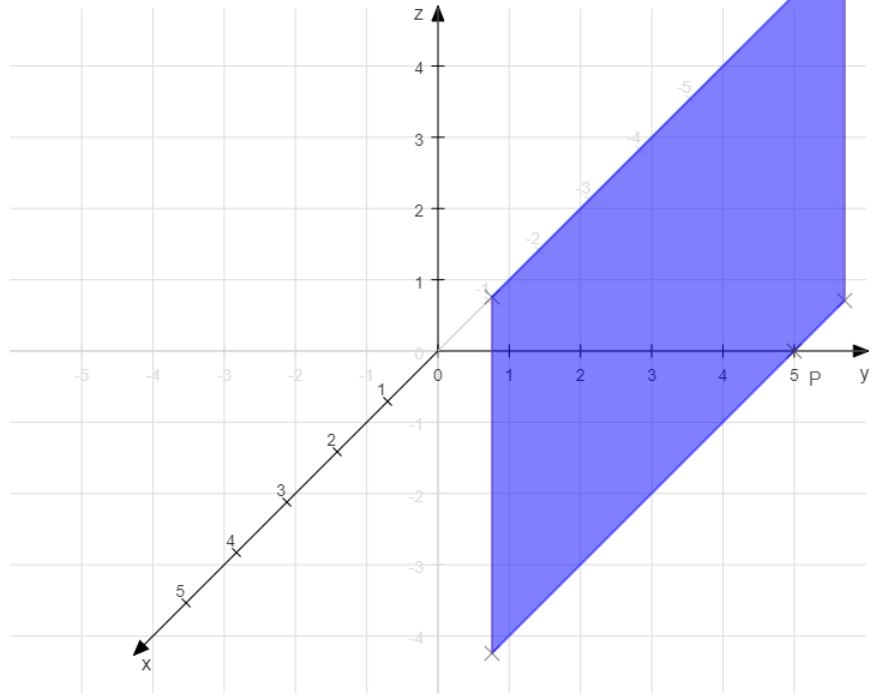
\includegraphics[scale=0.45]{Bilder/S72N2c.jpg}\\
			Die Ebene \(E\) hat also keinen Schnittpunkt mit der \(x_1x_3\)-Ebene.\\
			Damit ergibt sich die Ebene \colorbox{green!10}{\(E: x_2 = 5\)}
		\end{framed}
		\begin{framed}
			\noindent
			Wir wissen, die Koordinatengleichung einer Ebene hat folgende Form \colorbox{green!10}{\(E: \mathbf{a}x_1 + \mathbf{b}x_2 + \mathbf{c}x_3 = \mathbf{d}\)}.\\
			\par\noindent
			Um die Koordinatengleichung aufzustellen, setzen wir jeweils die gegebenen Punkte in die Gleichung ein und erhalten das dazugehörige lineare Gleichungssystem LGS (bestehend aus drei Gleichungen).\\
			\par\noindent
			Unter Anwendung des \textit{Gauß-Eliminations-Algorithmus} formen wir das LGS um und erhalten drei Gleichungen in Abhängigkeit der übrigen Unbekannten. Für diese Unbekannte wählen wir einen festen Wert und erhalten damit die übrigen drei Werte und können die Koordinatengleichung angeben.\\
			\hdashrule[0.5ex][x]{\textwidth}{0.1mm}{8mm 2pt}\\
			Siehe hierzu: S.71 Beispiel 3\\
		\end{framed}
		\begin{framed}
			\noindent
			\tiny{\color{codegray}\underline{S. 72 Nr. 5}}\\
			\normalsize\noindent
			Die Punkte \(A, B\) und \(C\) legen eine Ebene \(E\) fest. Bestimmen Sie eine Koordinatengleichung der Ebene.\\
			\textbf{(a)} \(A(0|2|-1), B(6|-5|0), C(1|0|1)\)\\
			Wir setzen also die Punkte in die Koordinatengleichung und erhalten folgendes LGS.
			\begin{tabularx}{\textwidth}{lllllllllll}
				I & \(\) & \(\) & \(+\) & \(2b\) & \(-\) & \(c\) & \(=\) & \(d\)\\
				II & \(\) & \(6a\) & \(-\) & \(5b\) & \(\) & \(\) & \(=\) & \(d\)\\
				III & \(\) & \(a\) & \(\) & \(\) & \(+\) & \(c\) & \(=\) & \(d\)\\
				\cline{1-9}\\
				\multicolumn{3}{c}{\(\mathbf{III + I}\)}\\
				I & \(\) & \(\) & \(+\) & \(2b\) & \(-\) & \(c\) & \(=\) & \(d\)\\
				II & \(\) & \(6a\) & \(-\) & \(5b\) & \(\) & \(\) & \(=\) & \(d\)\\
				III' & \(\) & \(a\) & \(+\) & \(2b\) & \(\) & \(\) & \(=\) & \(2d\)\\
				\cline{1-9}\\
				\multicolumn{3}{c}{\(\mathbf{5\cdot III' + 2\cdot II}\)}\\
				I & \(\) & \(\) & \(+\) & \(2b\) & \(-\) & \(c\) & \(=\) & \(d\)\\
				II & \(\) & \(6a\) & \(-\) & \(5b\) & \(\) & \(\) & \(=\) & \(d\)\\
				III & \(\) & \(17a\) & \(\) & \(\) & \(\) & \(\) & \(=\) & \(12d\) \(\Rightarrow\) \colorbox{green!10}{\(a = \frac{12}{17}d\)}\\
				\cline{1-9}\\
				& \multicolumn{9}{l}{\(a\) in II einsetzen}\\
				I & \(\) & \(\) & \(+\) & \(2b\) & \(-\) & \(c\) & \(=\) & \(d\)\\
				II & \(\) & \(6\cdot \frac{12}{17}d\) & \(-\) & \(5b\) & \(\) & \(\) & \(=\) & \(d\)& | \(-\frac{72}{17}d\)\\
			\end{tabularx}
			\begin{tabularx}{\textwidth}{llllllllll}
				& \(\) & \(\) & \(-\) & \(5b\) & \(\) & \(\) & \(=\) & \(-\frac{55}{17}d\)& | \(:(-5)\)\\
				& \(\) & \(\) & \(\) & \(b\) & \(\) & \(\) & \(=\) & \(\frac{11}{17}d\) & \(\Rightarrow\) \colorbox{green!10}{\(b = \frac{11}{17}d\)}\\
				\cline{1-9}\\
				& \multicolumn{9}{l}{\(b\) in I einsetzen}\\
				I & \(\) & \(\) & \(+\) & \(2\cdot\left(\frac{11}{17}d\right)\) & \(-\) & \(c\) & \(=\) & \(d\) & | \(-\frac{22}{17}d\)\\
				& \(\) & \(\) & \(\) & \(\) & \(-\) & \(c\) & \(=\) & \(-\frac{5}{17}d\) & |\(\cdot(-1)\)\\
				& \(\) & \(\) & \(\) & \(\) & \(\) & \(c\) & \(=\) & \(\frac{5}{17}d\) & \(\Rightarrow\) \colorbox{green!10}{\(c = \frac{5}{17}d\)}\\
			\end{tabularx}\\
			\par\bigskip\noindent
			Wir wissen nun: \colorbox{green!10}{\(a = \frac{12}{17}d\)}, \colorbox{green!10}{\(b = \frac{11}{17}d\)} und \colorbox{green!10}{\(c = \frac{5}{17}d\)}.\\
			Die Unbekannten \(a, b\) und \(c\) sind abhängig von \(d\). Wir wählen also nun \colorbox{blue!5}{\(d = 17\)}.\\
			\(\Rightarrow\) \colorbox{green!10}{\(a = 12\)}, \colorbox{green!10}{\(b =11\)} und \colorbox{green!10}{\(c = 5\)}\\
			Damit ergibt sich die Koordinatengleichung: \colorbox{green!10}{\(E: 12x_1 +11x_2 +5x_3 = 17\)}\\
			\par\bigskip\noindent
			\textbf{(b)} \(A(7|2|-1), B(4|1|3), C(1|3|2)\)\\
			Auch diesmal setzen wir die bekannten Punkte wieder in die Koordinatengleichung ein, wenden den Gauß-Algorithmus an und stellen so drei Variablen in Abhängigkeit der vierten Variablen dar.\\
			\begin{tabularx}{\textwidth}{lllllllllll}
				I & \(\) & \(7a\) & \(+\) & \(2b\) & \(-\) & \(c\) & \(=\) & \(d\)\\
				II & \(\) & \(4a\) & \(+\) & \(b\) & \(+\) & \(3c\) & \(=\) & \(d\)\\
				III & \(\) & \(a\) & \(+\) & \(3b\) & \(+\) & \(2c\) & \(=\) & \(d\)\\
				\cline{1-9}\\
				\multicolumn{3}{c}{\(\mathbf{I - 7\cdot III}\)}\\
				I' & \(\) & \(\) & \(-\) & \(19b\) & \(-\) & \(15c\) & \(=\) & \(-6d\)\\
				II & \(\) & \(4a\) & \(+\) & \(b\) & \(+\) & \(3c\) & \(=\) & \(d\)\\
				III & \(\) & \(a\) & \(+\) & \(3b\) & \(+\) & \(2c\) & \(=\) & \(d\)\\
				\cline{1-9}\\
				\multicolumn{3}{c}{\(\mathbf{II - 4\cdot III}\)}\\
				I' & \(\) & \(\) & \(-\) & \(19b\) & \(-\) & \(15c\) & \(=\) & \(-6d\)\\
				II' & \(\) & \(\) & \(-\) & \(11b\) & \(-\) & \(5c\) & \(=\) & \(-3d\)\\
				III & \(\) & \(a\) & \(+\) & \(3b\) & \(+\) & \(2c\) & \(=\) & \(d\)\\
				\cline{1-9}\\
				\multicolumn{3}{c}{\(\mathbf{I' - 3\cdot II'}\)}\\
				I' & \(\) & \(\) & \(\) & \(14b\) & \(\) & \(\) & \(=\) & \(3d\) & \(\Rightarrow\) \colorbox{green!10}{\(b = \frac{3}{14}d\)}\\
				II' & \(\) & \(\) & \(-\) & \(11b\) & \(-\) & \(5c\) & \(=\) & \(-3d\)\\
				III & \(\) & \(a\) & \(+\) & \(3b\) & \(+\) & \(2c\) & \(=\) & \(d\)\\
				\cline{1-9}\\
				& \multicolumn{9}{l}{\(b\) in II' einsetzen}\\
			\end{tabularx}
			\begin{tabularx}{\textwidth}{lllllllllll}
				II' & \(\) & \(\) & \(-\) & \(11\cdot \left(\frac{3}{14}d\right)\) & \(-\) & \(5c\) & \(=\) & \(-3d\) & |\(+\frac{33}{14}d\)\\
				& \(\) & \(\) & \(\) & \(\) & \(-\) & \(5c\) & \(=\) & \(-\frac{9}{14}d\) & |\(:(-5)\)\\
				& \(\) & \(\) & \(\) & \(\) & \(\) & \(c\) & \(=\) & \(\frac{9}{70}d\) & \(\Rightarrow\) \colorbox{green!10}{\(c = \frac{9}{70}d\)}\\
				\cline{1-9}\\
				& \multicolumn{9}{l}{\(b\) und \(c\) in III einsetzen}\\
				III & \(\) & \(a\) & \(+\) & \(3\cdot \left(\frac{3}{14}d\right)\) & \(+\) & \(2\cdot \left(\frac{9}{70}d\right)\) & \(=\) & \(d\) & |\((-\frac{9}{14}d); (-\frac{18}{70}d)\)\\
				& \(\) & \(a\) & \(\) & \(\) & \(\) & \(\) & \(=\) & \(\frac{1}{10}d\) & \(\Rightarrow\) \colorbox{green!10}{\(a = \frac{1}{10}d\)}\\
				\cline{1-9}\\
			\end{tabularx}
			\par\bigskip\noindent
			Wir wissen nun: \colorbox{green!10}{\(a = \frac{1}{10}d\)}, \colorbox{green!10}{\(b = \frac{3}{14}d\)} und \colorbox{green!10}{\(c = \frac{9}{70}d\)}.\\
			Man erkennt, die Variablen \(a, b\) und \(c\) sind nur von \(d\) abhängig. Wir wählen also nun \colorbox{blue!5}{\(d = 70\)}.\\
			\(\Rightarrow\) \colorbox{green!10}{\(a = 7\)}, \colorbox{green!10}{\(b =15\)} und \colorbox{green!10}{\(c = 9\)}\\
			Damit ergibt sich die Koordinatengleichung: \colorbox{green!10}{\(E: 7x_1 +15x_2 +9x_3 = 70\)}\\
		\end{framed}
	\end{worksheet}
\end{document}